\documentclass[CJKmath=true,10pt]{MyBook}


\usepackage{graphicx,float}
\usepackage{fontawesome5}
\usepackage[normalem]{ulem}
\usepackage{tikz}
\usetikzlibrary{arrows.meta, calc, patterns,angles,quotes,decorations}

\usepackage{siunitx}


\newcommand{\cgc}[3][]{
\begin{figure}[H]
\centering
\includegraphics[#1]{#2}
\caption{#3}
\end{figure}}

%设置一些字体
\usepackage{fontspec}
%\setCJKmainfont{Source Han Serif CN}
%[
%	Path=./fonts/hz/,
%	UprightFont = SourceHanSerifCN-Regular,
%	BoldFont = SourceHanSerifCN-Bold,
%	%ItalicFont = SourceHanSerifCN-Regular,
%	%BoldItalicFont = SourceHanSerifCN-Bold
%]
%\setCJKsansfont{Noto Sans CJK SC}
%[
%	Path=./fonts/hz/,
%	UprightFont = NotoSansCJKsc-Regular,
%	BoldFont = NotoSansCJKsc-Bold,
%	%ItalicFont = *-Regular,
%	%BoldItalicFont = *-Bold
%]
%\setCJKmonofont{Noto Sans Mono CJK SC}
%[
%UprightFont = *-Regular,
%BoldFont = *-Bold,
%AutoFakeSlant = 0.2
%]


% 定义 PowerShell 代码样式
\lstdefinelanguage{PowerShell}{
	keywords={Get-ChildItem, Rename-Item, -NewName, -replace, -WhatIf},
	morekeywords={Wait-Process, Get-Process},
	sensitive=false,
	morecomment=[l]{\#},
	morestring=[b]",
	morestring=[b]'
}

\lstset{
	language=PowerShell,
	basicstyle=\ttfamily\small,
	keywordstyle=\color{blue!80!black}\bfseries,
	stringstyle=\color{green!40!black},
	commentstyle=\color{gray}\itshape,
	frame=shadowbox,
	rulesepcolor=\color{gray!20},
	breaklines=true,
	showstringspaces=false,
	backgroundcolor=\color{gray!5}
}

\newcommand{\cuo}{\protect\textbf{\textcolor{red}{\ \faTimes\ \relax}}}
\newcommand{\dui}{\protect\textbf{\textcolor{green}{\ \faCheck\ \relax}}}

\begin{document}

%\frontmatter\tableofcontents
\mainmatter
%\setchapterimage{./images/055}
\setchapterimage{./images/bw}

\chapter{斜面}
如图\ref{lean.1}所示，质量为M、倾角$\theta$的粗糙斜面上，有一质量为m的木块以初速度$v_0$、加速度$a$匀加速下滑，M始终静止，重力加速度为$g$。则下滑过程地面对M的支持力大小为\uline{$\qquad\qquad$}，摩擦力大小为\uline{$\qquad\qquad$}，方向：\uline{$\qquad\qquad$}。
\begin{figure}[H]
	\centering
	\begin{tikzpicture}[>=Stealth,every node/.style={font=\small\itshape}]
		\def\ang{30}
		\def\len{4cm}
		\def\arclen{5mm}
		
		\coordinate (O)at(0,0);
		\coordinate (A)at(\len,0cm);
		\coordinate (B)at(0cm,{\len*tan(\ang)});
		\draw[fill=gray!5] (O)--(A)--(B)--cycle;
		\draw[thick] ($(A)-(\arclen,0mm)$)arc(180:180-\ang:\arclen)node[left,midway]{$\theta$};
		
		\coordinate (Box) at (1.5, {2.5*tan(\ang)});
		\begin{scope}[shift={(Box)},rotate=-\ang]
			\draw[fill=brown!40] (-0.35,0) rectangle (0.35,0.4);
			\node[rotate=-\ang] at (0,0.2) {$m$};
			\draw[->,thick] (0.4,0.2)--(1.2,0.2)node[rotate=-\ang,above,midway]{$a$};
		\end{scope}
		%绘制地面
		\path[pattern=north east lines] (-5mm,-2mm) rectangle (\len+5mm,-0.1mm); % 地面
		\node at(2cm,-0.5cm){水平地面};
	\end{tikzpicture}
	\caption{下滑}
	\label{lean.1}
\end{figure}
\begin{figure}[H]
	\centering
	\begin{tikzpicture}[>=Stealth]
		\def\ang{30}
		\def\len{4cm}
		\coordinate (Box) at (0, 0);
		\begin{scope}[shift={(Box)},rotate=-\ang]
			\draw[fill=brown!40] (-0.35,0) rectangle (0.35,0.4);
			\node[rotate=-\ang] at (0,0.2) {$m$};
			\draw[->,thick,dotted,red,rotate=\ang](-2cm,0.2cm)--(2cm,0.2cm)node[right]{$x'$};
			\draw[->,thick,dotted,red,rotate=\ang](0cm,-2cm)--(0cm,2cm)node[above]{$y'$};
			\draw[->,thick] (0.4,0.2)--(1.5,0.2)node[rotate=-\ang,above,midway]{$a$};
		\end{scope}
	
	\end{tikzpicture}
\end{figure}
\chapter{传送带}
\begin{examplebox}
将粉笔头A轻放在以$v_0=2\mathrm{m/s}$的恒定速度运动的足够长的水平传送带上后，传送带上留下一条长度为$x=4\mathrm{m}$的划线。若使该传送带改做加速度大小为$a_0=1.5\mathrm{m/s^2}$的匀减速运动直至速度为0，并且在传送带开始做匀减速运动的同时，将另一相同材质的粉笔头B轻放在传送带上，重力加速度$g=10\mathrm{m/s^2}$。求：
\begin{enumerate}
	\item 粉笔头 B 停止在传送带上的位置与划线起点间的距离$d$为多少？
	\item  粉笔头 B 在传送带上的划痕 $s$	有多长？
\end{enumerate}

\end{examplebox}
根据A的划痕由$v^2=2ax\iff a=\dfrac{1}{2}=\mu g$，此为粉笔的加速度。粉笔$B$轻放在传送带上，在达到共速前做匀加速直线运动，加速度为刚才求的$a$，设共速时刻为t，则：$2-a_0t=at\Rightarrow t=0.8$，此时$v_共=0.8m/s$。

共速后，粉笔的加速度$0.8<1.5$，因此\textbf{不能}\footnote{滑动摩擦力约等于最大静摩擦力，最大静摩擦力提供的加速度就是a，小于传送带的加速度$a_0$。}和传送带一起匀减速到0，粉笔以原来的加速度减速到0，传送带以-1.5的加速度减速到0。：
\begin{figure}[H]\centering
	\begin{tikzpicture}[scale=1.5,>=Stealth,every node/.style={font=\small\itshape}]
		\def\len{3cm}
		\def\v{2cm}
		
		\coordinate (O)at(0,0);
		\coordinate (A)at(\len,0cm);
		\coordinate (B)at(0cm,\len);
		
		\draw [thick,black,->](O)--(A)node[right]{$t$};
		\draw [thick,black,->](O)--(B)node[above]{$v$};
		
		\draw[thick,red](0,\v)node[left]{$v_0$}--(4/3,0)node[near start,above,sloped]{传送带};
		\draw[thick,red](0,0)--(0.8,0.8)--(1.8,0);
		
		\path[pattern=crosshatch dots light steel blue](0,2)--(0.8,0.8)--(O)--cycle;
		\path[pattern=crosshatch dots light steel blue](4/3,0)--(0.8,0.8)--(1.8,0)--cycle;
	\end{tikzpicture}
	\caption{$V-T$图}
\end{figure}







\chapter{牛二}
如图\ref{fig3.1}所示，质量为10 kg的物体\( A \)拴在一个被水平拉伸的弹簧一端，弹簧的拉力为5 N时，物体\( A \)处于静止状态。若小车突然以\( 0.8 m/s^2 \)的加速度向右加速运动，重力加速度\( g = 10 m/s^2 \)，则（）
\begin{enumerate}[label=\Alph*.\ ]
	\item 物体\( A \)可能会相对小车向右运动
	\item  物体\( A \)受到的弹簧的拉力可能增大
	\item  物体\( A \)受到的摩擦力大小可能不变
	\item  物体\( A \)受到的摩擦力一定减小
\end{enumerate}

\begin{figure}[H]
	\begin{center}
		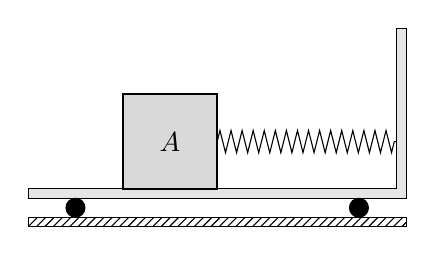
\begin{tikzpicture}[scale=1.2]
			% 小车
			\draw[fill=gray!20] (0,-0.8)--(4,-0.8)--(4,-0.7)--(4,1)--(3.9,1)--(3.9,-0.7)--(0,-0.7)--cycle;
			\draw[fill] (0.5,-0.9) circle (0.1);
			\draw[fill] (3.5,-0.9) circle (0.1);
			\draw[pattern=north east lines] (0,-1.1) rectangle (4,-1); % 地面
			
			% 物体A
			\draw[fill=gray!30,thick] (1,-0.7) rectangle (2,0.3);
			\node at (1.5,-.2) {$A$};
			
			% 弹簧coil也可以
			\draw[decorate,decoration={zigzag, segment length=4pt, amplitude=4pt}] (2,-0.2) -- (3.9,-0.2);
			
		\end{tikzpicture}
	\end{center}
	\caption{习题}
	\label{fig3.1}
\end{figure}

\subsection*{解答}

\textbf{推理：}原来拉力$5N$静止不动，表示$f_{max静摩擦力}\ge 5N$。现在突然需要向右$8N$的力，弹簧不是瞬时力，只能提供$5N$，那么必定有$3N$水平向右的力，由静摩擦力提供。此时物体A：$f_{摩擦力} <  f_{max摩擦力}$不会动。
\begin{enumerate}
	
	
	\item 		\textbf{初始状态分析：}
	由图可知，弹簧连接在物体\( A \)的右侧和小车的右壁之间，且弹簧处于“被拉伸”状态，因此弹簧对物体\( A \)施加向右的拉力 \( F_{\text{弹}} = 5 \text{ N} \)。
	
	物体\( A \)处于静止状态，受力平衡。在水平方向上：
	\begin{align*}
		&\because F_{\text{弹}} + f = 0 \\
		&\therefore f = -F_{\text{弹}} = -5 \text{ N}
	\end{align*}
	即初始摩擦力大小为 5 N，方向水平向左。
	
	同时可知，最大静摩擦力 \( f_{\max} \) 至少能提供 5 N 的力，即 \( f_{\max} \geq 5 \text{ N} \)。
	
	\item 		\textbf{加速状态分析：}
	小车以 \( a = 0.8 \text{ m/s}^2 \) 向右加速。假设物体\( A \)相对于小车静止（即随车一起加速），则物体\( A \)的加速度也是 \( 0.8 \text{ m/s}^2 \)（向右）。
	
	根据牛顿第二定律，物体\( A \)所受合外力应为：
	\[ F_{\text{合}} = ma = 10 \times 0.8 = 8 \text{ N} \text{（向右）} \]
	
	此时，水平方向受力仍为弹簧拉力和摩擦力。根据假设相对静止，弹簧长度未变，拉力仍为 \( 5 \text{ N} \)（向右）。
	设此时的摩擦力为 \( f' \)（向右为正）：
	\[ F_{\text{弹}} + f' = F_{\text{合}} \]
	\[ 5 + f' = 8 \]
	\[ f' = 3 \text{ N} \]
	
	结果表明，要使物体随车一起以 \( 0.8 \text{ m/s}^2 \) 加速，需要 3 N 向右的静摩擦力。
	
	\item 		\textbf{检验假设：}
	我们算出需要的静摩擦力为 3 N。而我们已知最大静摩擦力 \( f_{\max} \geq 5 \text{ N} \)。
	因为 \( 3 \text{ N} < 5 \text{ N} \)，所以静摩擦力足以提供所需的加速度，物体\( A \) \textbf{不会} 发生相对滑动，确实和小车保持相对静止。
	
	\item 		\textbf{对比前后状态：}
	\begin{itemize}
		\item \textbf{弹簧拉力：} 始终为 5 N（因为没有相对滑动）。
		\item \textbf{摩擦力：} 由 5 N（向左）变为 3 N（向右）。
		\item \textbf{摩擦力大小：} 由 5 N 减小为 3 N。
	\end{itemize}
	
	\item 		\textbf{选项分析：}
	\begin{itemize}
		\item \textbf{A. 物体\( A \)可能会相对小车向右运动}：
		\cuo 我们已经验证物体相对于小车静止。即使发生滑动，物体相对于小车的加速度小于车的加速度，表现为相对后退（向左），绝不可能相对向右冲去。
		\item \textbf{B. 物体\( A \)受到的弹簧的拉力可能增大}：
		\cuo 物体相对静止，弹簧形变量不变，拉力不变。
		\item \textbf{C. 物体\( A \)受到的摩擦力大小可能不变}：
		\cuo。摩擦力大小由 5 N 变为 3 N，一定变了。
		\item \textbf{D. 物体\( A \)受到的摩擦力一定减小}：
		\dui 大小从 5 N 变为 3 N，确实减小了。
	\end{itemize}
\end{enumerate}
\textbf{答案：D}

如图\ref{fig3.2}所示，质量分别为 $m_A$ 和 $m_B$ 的 A、B 两物体沿着固定光滑斜面匀加速下滑，斜面倾角为 $\theta=30^\circ$，A 的上表面水平，且 A、B 始终保持相对静止，重力加速度为 $g$。则物体 A、B 的加速度大小为：\underline{$g\sin\theta$}；B 受到 A 的摩擦力大小为：\underline{$M_B\sin\theta\cos\theta=\dfrac{\sqrt{3}}{4}M_B\cdot g$}、B 受到 A的支持力大小为：\underline{$M_Bg-N=M\cdot a\sin\theta\iff N=\dfrac{3}{4}m_Bg$}。
\begin{figure}[H]
	\centering
	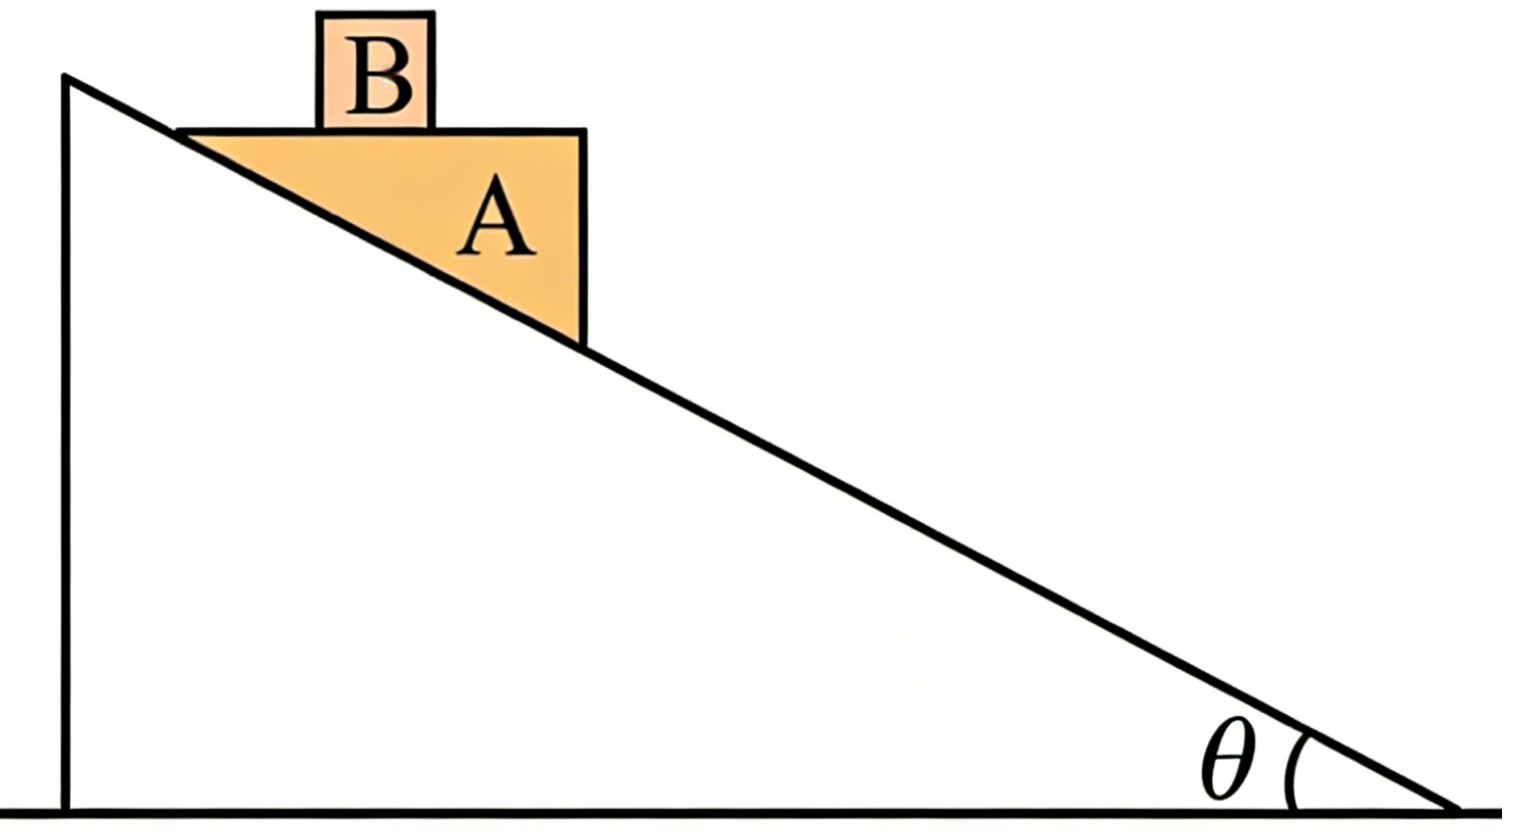
\includegraphics[width=5cm]{pics/2.png}
	\caption{物体匀加速下滑示意图}
	\label{fig3.2}
\end{figure}
加速度有竖直向下分量，物体失重。

(多选)如图所示，物体A的质量为$M$，水平面光滑，不计滑轮的质量及摩擦。当在轻绳的$B$端挂一质量为$m$的物体时，物体$A$的加速度为$a_1$；当在轻绳的$B$端施以$F=mg$的竖直向下的拉力作用时，$A$的加速度为$a_2$，则（）

\begin{enumerate}
	\item[A.] $a_1=\dfrac{m}{M}g$
	\item[B.] $a_2=\dfrac{m}{M}g$
	\item[C.] $a_1=a_2$
	\item[D.] $a_1<a_2$
\end{enumerate}

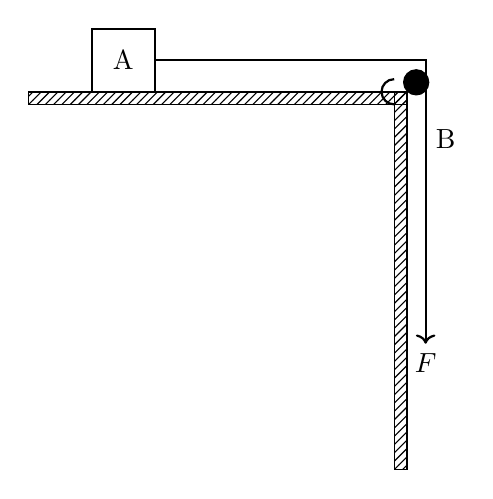
\begin{tikzpicture}[scale=0.8]
	% 绘制水平面和竖直墙面
	\draw[thick] (0,0) -- (6,0);
	\draw[thick] (6,0) -- (6,-6);
	\draw[pattern=north east lines] (0,-0) rectangle (6,-0.2);
	\draw[pattern=north east lines] (6,0) rectangle (5.8,-6);
	
	% 绘制物体A
	\draw[thick] (1,0) rectangle (2,1) node[midway] {A};
	
	% 绘制滑轮
	\filldraw[black] (6.15,0.15) circle (0.2);
	\draw[thick] (5.8,-0.2) arc (270:90:0.2);
	
	% 绘制绳子
	\draw[thick] (2,0.5) -- (6.3,0.5)  -- (6.3,-2) node[midway, right] {B};
	
	% 绘制拉力F
	\draw[thick, ->] (6.3,-2) -- (6.3,-4) node[below] {$F$};
\end{tikzpicture}
\end{document}